\subsection{Publicações}
Para as \textbf{Publicações} da série \ppod foi criado um \gls{cpt} do Wordpress, chamado ``\textit{publicacao\_post\_type}'', e as diversas páginas necessárias (\textit{archive-publicacao.php}, \textit{content-publicacao.php}, \textit{publicacao-card.php}, \textit{sidebar-publicacao.php} e \textit{single-publicacao.php}). O \gls{cpt} criado pode ser observado no arquivo \textit{functions.php} do projeto \textit{pensandoodireito-tema}\footnote{Arquivo \textit{functions.php} do projeto \textit{pensandoodireito-tema} no github: \url{https://github.com/pensandoodireito/pensandoodireito-tema/blob/master/functions.php}}.

\subsubsection*{Página Principal}
Para as \textbf{Publicações} da série \ppod foi desenvolvida uma área dedicada, conforme pode ser observado na Figura \ref{fig:publicacoes-geral}.

\begin{figure}[Htb]%
	\begin{center}
		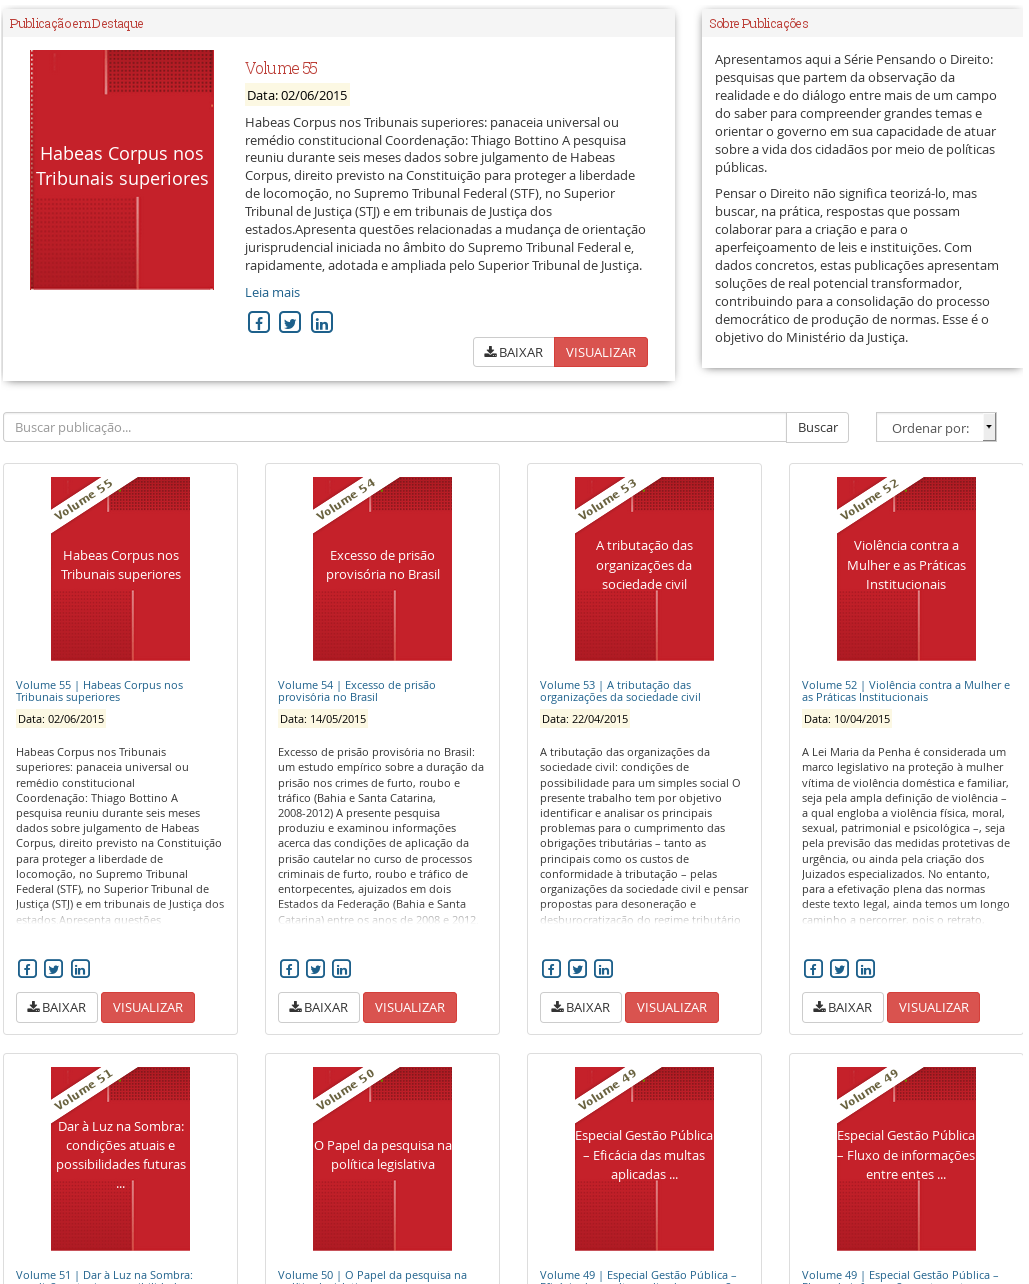
\includegraphics[scale=0.36]{./imagens/publicacoes-geral.png}%
	\end{center}%
	\caption{Página das Publicações\label{fig:publicacoes-geral}}%
	%\fonte{\url{http://participacao.mj.gov.br/}}%
\end{figure}%

Nesta área são apresentadas todas as publicações já disponibilizadas, com um destaque para a publicação mais recente - Figure \ref{fig:publicacoes-destaque}; e as demais em fileiras de 4 publicações, conforme pode ser observado na Figura \ref{fig:publicacoes-matriz}. As publicações nas fileiras serão apresentadas, por padrão, em ordem de publicação, da mais nova para a mais antiga.

\begin{figure}[htb]%
	\begin{center}
		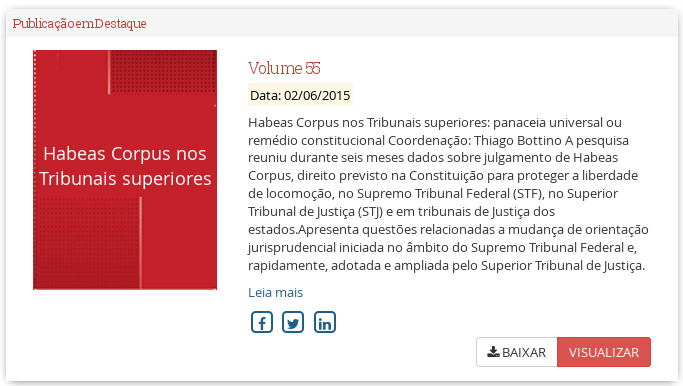
\includegraphics[scale=0.44]{./imagens/publicacoes-destaque.png}%
	\end{center}%
	\caption{Publicação em Destaque\label{fig:publicacoes-destaque}}%
	%\fonte{\url{http://participacao.mj.gov.br/}}%
\end{figure}%

Também há disponível a possibilidade de o usuário filtrar as publicações por meio de uma busca textual e mudar a regra de ordenação das publicações (por nome ou por número da publicação), conforme a Figura \ref{fig:publicacoes-busca}.

\begin{figure}[htb]%
	\begin{center}
		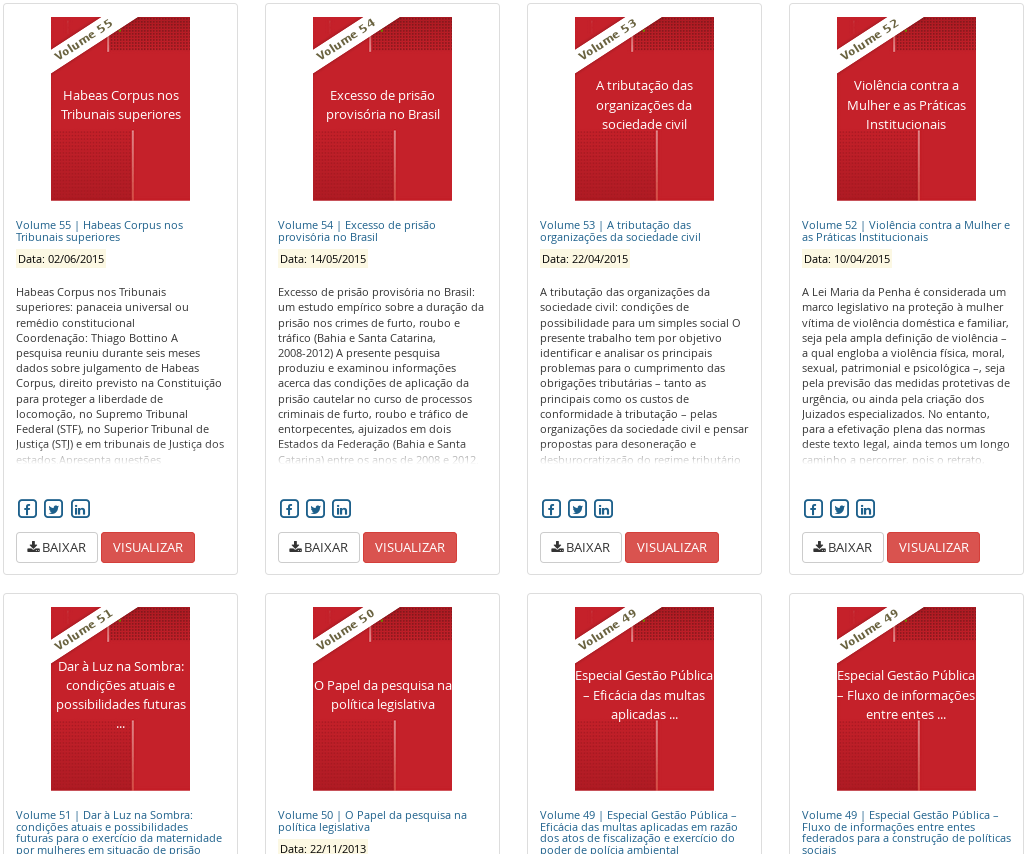
\includegraphics[scale=0.31]{./imagens/publicacoes-matriz.png}%
	\end{center}%
	\caption{Demais Publicações\label{fig:publicacoes-matriz}}%
	%\fonte{\url{http://participacao.mj.gov.br/}}%
\end{figure}%

Uma funcionalidade que não foi implementada, mas que sugere-se adicionar é o recurso que permita ao usuário escolher se deseja a ordenação das publicações apresentadas de forma ``crescente'' ou ``decrescente''. Uma boa solução seria utilizar a simbologia de setas para cima ou para baixo ao lado da caixa de seleção do tipo de ordenação que o usuário deseja. Esta sugestão foi registada como \textit{issue} de número 240\footnote{\textit{Issue} criada: \url{https://github.com/pensandoodireito/participacao-sitebase/issues/240}} no repositório de gestão do projeto\footnote{Repositório de gestão do projeto: \url{https://github.com/pensandoodireito/participacao-sitebase/issues}}.

Para melhorar a usabilidade e o desempenho para os usuários, inicialmente serão mostradas apenas as 9 publicações mais recentes - incluso o destaque; e ao final das mesmas é apresentado um botão "Mais Publicações" que irá carregar, dinâmicamente, mais uma fileira de 4 publicações a cada clique sobre o botão.

\begin{figure}[htb]%
	\begin{center}
		
\includegraphics[scale=0.55]{./imagens/publicacoes-busca.png}%
	\end{center}%
	\caption{Busca das Publicações\label{fig:publicacoes-busca}}%
	%\fonte{\url{http://participacao.mj.gov.br/}}%
\end{figure}%

\subsubsection*{Página da Publicação}
Já na página de uma publicação específica, há um \textit{widget} ``outras publicações'', que traz outras publicações da série \ppod que versem sobre temáticas semelhantes ou que dialoguem com a publicação sendo visualizada. É preciso verificar o critério atual de escolhe destas publicações.

Nesta página há a possibilidade de o usuário visualizar o PDF da publicação na própria página, ler um resumo sobre a publicação, baixar o PDF da mesma, compartilhá-la nas redes sociais (Facebook, Twitter ou LinkedIn), ver os autores e autoras da Publicação e navegar para a publicação anterior ou para a próxima, caso elas existam.

Com relação ao compartilhamento nas redes sociais, é preciso verificar se as meta-informações da página estão configuradas de forma que o compartilhamento na rede social apresente uma imagem, além do texto, visto que a utilização de imagem aumenta o impacto da publicação nas redes sociais.

Sobre a visualização de autoras e autores, este recurso não foi completamente implementado pois não foi desenvolvido um campo específico para tal conteúdo.

A previsão inicial era de que os autores da publicação seriam apresentado junto a uma mini-biografia dos mesmos. Porém, não há na ferramenta um ``catálogo de autores'', que permita cadastrar previamente os autores e reutilizar esse cadastro. Dessa forma, a única solução mais direta seria a implementação de um campo extra (um \textit{array} num campo do tipo \textit{meta} do \gls{cpt}) que permita, a cada publicação, inserir o/a(s) autor(es)/autora(s)
e sua respectiva descrição. Esta abordagem não foi implementada por falta de tempo para o desenvolvimento da mesma e também pois ela demandaria recadastrar esta informação para todas as publicações já existentes na plataforma, mas recomenda-se que esta abordagem seja seguida. Após sua implementação no \textit{backend}, será necessário também implementá-la no front-end, criando a tela que apresentará este conteúdo, após o clique no link ``Ver autores'' que se apresenta logo acima dos botões de redes sociais. 

\subsubsection*{\textit{Widget} Publicações}
Foi desenvolvido um \gls{widget} para as publicações, que permite a inclusão de um \gls{sidebar} que faz referências a ``outras publicações'', conforme observado na figura \ref{fig:publicacoes-sidebar}.

A proposta deste \gls{widget} é ser utilizado na página que apresenta uma única publicação, trazendo outras publicações da série \ppod que versem sobre temáticas semelhantes ou que dialoguem com a publicação sendo visualizada.

É preciso verificar o critério atual de escolhe destas publicações.

\begin{figure}[htb]%
	\begin{center}
		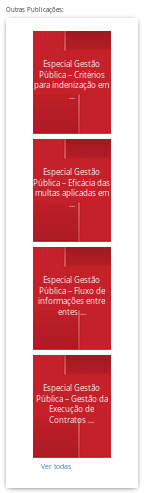
\includegraphics[scale=0.55]{./imagens/publicacoes-sidebar.png}%
	\end{center}%
	\caption{Sidebar das Publicações\label{fig:publicacoes-sidebar}}%
	%\fonte{\url{http://participacao.mj.gov.br/}}%
\end{figure}%
